%%
%%############################
\newcommand{\prexo}{\emph{pre\_exodus \,}}
\newcommand{\bc}{\emph{bc-file \,}}
\newcommand{\head}{\emph{header-file \,}}

\chapter{FSI Tutorial 3d with \prexo and Cubit}
\label{tut_fsi_preexo:chap}

%%
%%============================
\section{Introduction}

As example, we consider a 3d driven cavity example as
sketched in Fig. \ref{tut_fsi_preexo:1.1} with a depth of 0.05.
Hint: In case you want or need to see a sample solution for this tutorial 
you will find corresponding files in the \baci{} subfolder \emph{/tests/framework-tests/}!
However, it is highly recommended to look at these files only in case you encounter severe problems
while stepping through the tutorial.\\
For further details and references we refer the reader to:\\
W.A. Wall, PhD thesis, 1999
(available under \texttt{/lnm/literature/1999/})

\begin{figure}[h]
\hfil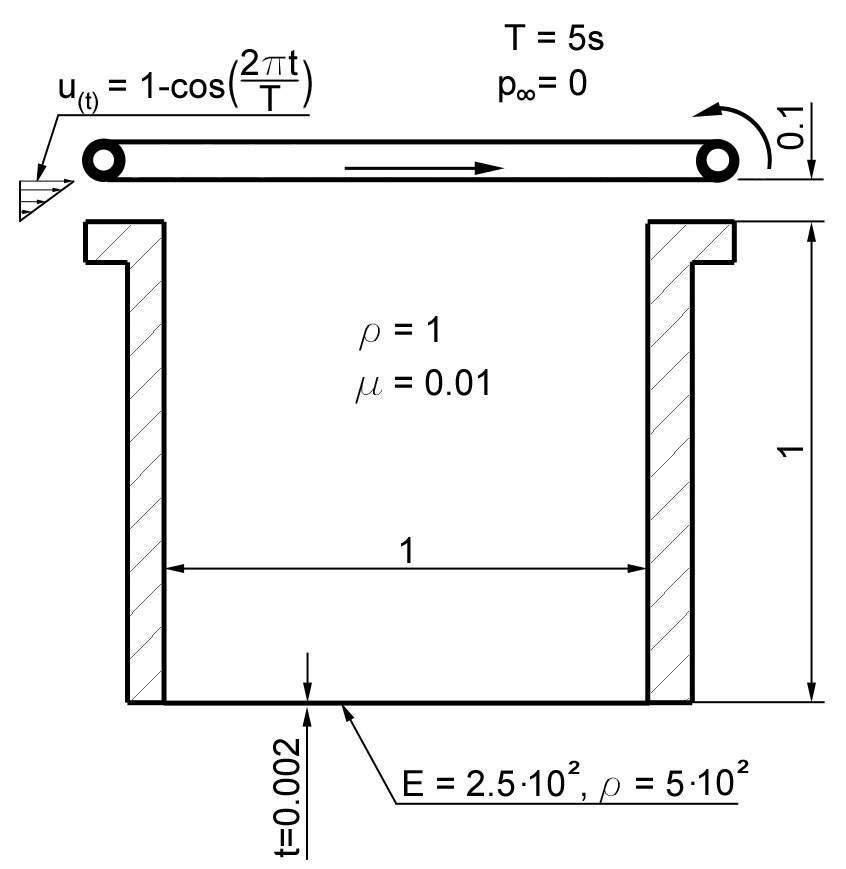
\includegraphics[scale=0.2]{Bilder/Angabeskizze}

\caption{\label{tut_fsi_preexo:1.1} The driven cavity example}
\end{figure}

\section{Creating the Geometry with Cubit}

Besides meshing cubit also has several geometry creation methods. We refer
to the provided manual and tutorials. It supports scripting (also Python),
therefore we provide the following \textit{Journal}-file containing the
necessary geometry commands as well as mesh and definitions for elements and
boundary conditions, respectively.

\begin{small} \begin{verbatim}
 reset

$=======================Define parameters
# {Depth=0.05}
# {Width=1.0}
# {BottomHeight=0.002}
# {CavityHeight=1.0}
# {InflowHeight=0.1}
# {MeshDepth=1}
# {MeshWidth=32}
# {MeshBottomHeight=1}
# {MeshCavityHeight=32}
# {MeshInflowHeight=7}

$$GEOMETRY
$=====================Create Bottom
brick x {Width} y {BottomHeight} z {Depth}
volume 1 move x {Width/2} y {-BottomHeight/2} z {-Depth/2}
$=====================Create Fluid Part
$ cavity + inflow
brick  x {Width} y {CavityHeight+InflowHeight} z {Depth}
align volume 2 surface 9 with surface 5
$ divide cavity and inflow region
webcut volume 2 with plane yplane offset {CavityHeight} imprint merge

$$MESHING
$=======================Mesh Bottom
curve 3 interval {MeshBottomHeight}
curve 3 scheme equal
mesh curve 3
curve 2 interval {MeshWidth}
curve 2 scheme equal
mesh curve 2
curve 11 interval {MeshDepth}
curve 11 scheme equal
mesh curve 11
mesh volume 1
$=======================Mesh Cavity
curve 29 interval {MeshCavityHeight}
curve 29 scheme equal
mesh curve 29
curve 16 interval {MeshWidth}
curve 16 scheme equal
mesh curve 16
curve 21 interval {MeshDepth}
curve 21 scheme equal
mesh curve 21
mesh volume 2
$=======================Mesh Inflow
curve 40 interval {MeshInflowHeight}
curve 40 scheme equal
mesh curve 40
mesh volume 3

$$EXODUS - definitions
$=======================Structure
block 1 volume 1
block 1 name "flexible bottom"
nodeset 1 surface 4
nodeset 1 name "structure surface left"
nodeset 2 surface 6
nodeset 2 name "structure surface right"
nodeset 3 surface 1
nodeset 3 name "structure surface front"
nodeset 4 surface 2
nodeset 4 name "structure surface back"
nodeset 5 surface 5
nodeset 5 name "structure coupling surface"
nodeset 6 curve 3
nodeset 6 name "structure edge front left"
nodeset 7 curve 7
nodeset 7 name "structure edge back left"
nodeset 8 curve 5
nodeset 8 name "structure edge back right"
nodeset 9 curve 1
nodeset 9 name "structure edge front right"
$=======================Fluid
block 2 volume 2 3
block 2 name "fluid"
nodeset 10 surface 15
nodeset 10 name "cavity wall left"
nodeset 11 surface 17
nodeset 11 name "cavity wall right"
nodeset 12 surface 14 21
nodeset 12 name "fluid wall front"
nodeset 13 surface 16 20
nodeset 13 name "fluid wall back"
nodeset 14 surface 9
nodeset 14 name "fluid coupling surface"
nodeset 15 surface 11
nodeset 15 name "lid"
nodeset 16 surface 22
nodeset 16 name "inflow"
nodeset 17 curve 29
nodeset 17 name "cavity edge front left"
nodeset 18 curve 31
nodeset 18 name "cavity edge back left"
nodeset 19 curve 32
nodeset 19 name "cavity edge back right"
nodeset 20 curve 30
nodeset 20 name "cavity edge front right"
nodeset 21 curve 16
nodeset 21 name "cavity edge front bottom"
nodeset 22 curve 18
nodeset 22 name "cavity edge back bottom"
nodeset 23 curve 21
nodeset 23 name "cavity edge left bottom"
nodeset 24 curve 22
nodeset 24 name "cavity edge right bottom"
nodeset 25 curve 26
nodeset 25 name "cavity-inflow edge"
nodeset 26 curve 40
nodeset 26 name "inflow edge front"
nodeset 27 curve 39
nodeset 27 name "inflow edge back"
nodeset 28 curve 23
nodeset 28 name "lid edge left"
nodeset 29 curve 14
nodeset 29 name "lid edge front"
nodeset 30 curve 20
nodeset 30 name "lid edge back"
nodeset 31 vertex 12
nodeset 31 name "cavity vertex front left bottom"
nodeset 32 vertex 15
nodeset 32 name "cavity vertex back left bottom"
nodeset 33 vertex 14
nodeset 33 name "cavity vertex back right bottom"
nodeset 34 vertex 9
nodeset 34 name "cavity vertex front right bottom"
nodeset 35 vertex 19
nodeset 35 name "cavity-inflow vertex front 1"
nodeset 36 vertex 17
nodeset 36 name "cavity-inflow vertex front 2"
nodeset 37 vertex 11
nodeset 37 name "lid vertex front left"
nodeset 38 vertex 16
nodeset 38 name "lid vertex back left"
\end{verbatim} \end{small}

Within Cubit, open the Journal-Editor (\emph{Tools}$\to$\emph{Journal
Editor}), paste the text above and press \emph{play}. For later usage it is convenient
to save the current content of the Journal-Editor into a \emph{*.jou} file. 
Export now the created geometry and mesh to an
exodus-file of your choice via \emph{File}$\to$\emph{Export...}. 
During export, set the dimension explicitly to 3d.

\section{Working with \prexo and \baci{}}

\prexo is a C++ code embedded into the \baci{} environment. It is meant to
transfer a given mesh into a \baci{}-readable input file.

\subsection{Preliminaries}

If not already done, compile \prexo via \begin{verbatim}make pre_exodus\end{verbatim} after 
configuring \baci{} in the usual way.

\subsection{General Procedure of Creating a Valid \baci{} Input File}
With a given mesh including some nodal clouds to apply conditions to you need
another text-file (\bc) where you specify, what you would like to do with
it. It contains for example the specific element declaration (fluid, structure,
parameters, etc.) and the particular boundary condition such as Dirichlet or
Neumann. Finally, a \head consists of general parameters such as
solvers, algorithmic parameters, etc. Those three files are merged by \prexo
into an input file for \baci{}. This file is then \emph{automatically} validated
using all available \baci{} validation and is therefore likely to run.

Sure, you usually don not have already a proper \head and matching \bc. By
typing
\begin{center}
  \verb|./pre_exodus --exo=yourmesh.e|
\end{center}
you get two preliminary files
'default.head' and 'default.bc'. The first contains the currently valid header
parameters with default values and commented options which you can edit to
adapt it to your means. Similarly, 'default.bc' consists of all your mesh
entities and a list of all currently valid conditions. See next section for
details how to work with it and how to get valid input files.

\subsection{Running a Simulation with \baci{}}
\label{tut_fsi_preexo:baci}
To start the solver use the call 
\begin{center}
	\verb|./baci-release [inputdirectory]/your_example.dat [outputdirectory]/outputprefix|
\end{center}
(in the \baci{}-directory). The results are then written to
the result directory with the prefix you chose.

\section{The Structure Part}

In the following we will always refer to the same exodus-file of the whole
geometry and mesh. For the different problems we differentiate between \head and
\bc. We start with the pure structural simulation.

\subsection{\head}
Find the following sections in 'default.head' and edit as given:

\begin{itemize}
 \item \verb|PROBLEM TYP|

 \verb|PROBLEMTYP Structure|

 \item \verb|STRUCTURAL DYNAMIC|

 \verb|DYNAMICTYP     GenAlpha|

 \verb|LINEAR_SOLVER 1|

 \verb|NUMSTEP 10|

 \verb|TIMESTEP 0.5|

 \item \verb|SOLVER 1|
 
 \verb|NAME Solver|

 \verb|SOLVER UMFPACK|

 \item \verb|MATERIALS|

  insert \verb|MAT 1 MAT_Struct_StVenantKirchhoff YOUNG 250.0 NUE 0.3 DENS 500|
 
\end{itemize}
Safe the file under a different name, e.g. 'dc\_struct.head'.


\subsection{\bc}
As mentioned above we create our \bc from the 'default.bc'. This consists of a
introduction part where some global mesh statistics are given, a couple of
example entries for definitions, a list of all defined mesh entities in
your mesh-file, and finally a list of all valid \baci{} conditions to choose
from.

For our structure problem we will only define the corresponding mesh entities. They are easily identified by the names you have given in Cubit, e.g. ``flexible bottom'', or ``inflow''. You may notice that we do not assign any 'E'-entity-numbering.
They are automatically determined in the order they appear in the \bc. Therefore, if you want to change the numbering in the \baci{} input file, e.g. for correct hierarchy, you have to change the order in the \bc.

Therefore we assign:
\begin{itemize}
 \item \verb|*eb1="ELEMENT"| \qquad the structure elements
 \begin{small} \begin{verbatim}
 sectionname="STRUCTURE"
 description="MAT 1 KINEM nonlinear EAS sosh8 ANS sosh8 THICKDIR auto"
 elementname="SOLIDSH8"
 \end{verbatim} \end{small}
 
 \item \verb|*ns1="CONDITION"| \qquad clamping
 \begin{small} \begin{verbatim}
sectionname="DESIGN SURF DIRICH CONDITIONS"
description="NUMDOF 3 ONOFF 1 1 1 VAL 0.0 0.0 0.0 CURVE none none none FUNCT 0 0 0"
 \end{verbatim} \end{small}
 
 \item \verb|*ns2="CONDITION"| \qquad clamping
 \begin{small} \begin{verbatim}
sectionname="DESIGN SURF DIRICH CONDITIONS"
description="NUMDOF 3 ONOFF 1 1 1 VAL 0.0 0.0 0.0 CURVE none none none FUNCT 0 0 0"
 \end{verbatim} \end{small}
 
 \item \verb|*ns3="CONDITION"| \qquad fix in z-direction
 \begin{small} \begin{verbatim}
sectionname="DESIGN SURF DIRICH CONDITIONS"
description="NUMDOF 3 ONOFF 0 0 1 VAL 0.0 0.0 0.0 CURVE none none none FUNCT 0 0 0"
 \end{verbatim} \end{small}
 
 \item \verb|*ns4="CONDITION"| \qquad fix in z-direction
 \begin{small} \begin{verbatim}
sectionname="DESIGN SURF DIRICH CONDITIONS"
description="NUMDOF 3 ONOFF 0 0 1 VAL 0.0 0.0 0.0 CURVE none none none FUNCT 0 0 0"
 \end{verbatim} \end{small}
 
 \item \verb|*ns5="CONDITION"| \qquad the later coupling surface is first loaded with constant vertical surface pressure
 \begin{small} \begin{verbatim}
sectionname="DESIGN SURF NEUMANN CONDITIONS"
description="none 0 1 0 0 0 0  0.0 -0.01 0.0 0.0 0.0 0.0  Live Mid 0 0 0 0 0 0"
 \end{verbatim} \end{small}
 
 \item \verb|*ns6="CONDITION"| \qquad hierarchically corresponding line condition
 \begin{small} \begin{verbatim}
sectionname="DESIGN LINE DIRICH CONDITIONS"
description="NUMDOF 3 ONOFF 1 1 1 VAL 0.0 0.0 0.0 CURVE none none none FUNCT 0 0 0"
 \end{verbatim} \end{small}
 
 \item \verb|*ns7="CONDITION"| \qquad hierarchically corresponding line condition
 \begin{small} \begin{verbatim}
sectionname="DESIGN LINE DIRICH CONDITIONS"
description="NUMDOF 3 ONOFF 1 1 1 VAL 0.0 0.0 0.0 CURVE none none none FUNCT 0 0 0"
 \end{verbatim} \end{small}
 
 \item \verb|*ns8="CONDITION"| \qquad hierarchically corresponding line condition
 \begin{small} \begin{verbatim}
sectionname="DESIGN LINE DIRICH CONDITIONS"
description="NUMDOF 3 ONOFF 1 1 1 VAL 0.0 0.0 0.0 CURVE none none none FUNCT 0 0 0"
 \end{verbatim} \end{small}
 
 \item \verb|*ns9="CONDITION"| \qquad hierarchically corresponding line condition
 \begin{small} \begin{verbatim}
sectionname="DESIGN LINE DIRICH CONDITIONS"
description="NUMDOF 3 ONOFF 1 1 1 VAL 0.0 0.0 0.0 CURVE none none none FUNCT 0 0 0"
 \end{verbatim} \end{small}

\end{itemize}

Delete the remaining items \verb|eb2| and \verb|ns10| to \verb|ns38|. \newline

For Dirichlet conditions the first entry specifies the global degree of freedom of the problem, denoted as $n$. The $n$ following entries are the flags specifying which degrees of freedom are to be prescribed in detail, where \verb|1| means Dirichlet condition is applied and \verb|0| corresponds to a free degree of freedom. In structure computations the flags two to four correspond to displacements in $x$, $y$ and $z$ direction, respectively. Flags five to seven are ignored here. The next six entries of the \verb|description| specify the values of the prescribed displacements. Subsequently six time dependent curve ids can be given, corresponding to the \verb|CURVE| section in the \head. Finally six spatial function ids can be defined, corresponding to the \verb|FUNCT| section in the \head. \verb|CURVE| and \verb|FUNCT| are evaluated and their values are multiplied with the values defined before. \newline

Safe the file under a different name, e.g. 'dc\_struct.bc'.

\subsection{Creating \baci{} Input File and Running the Simulation}
Run in a shell \verb|./pre_exodus --exo=dc.e --head=dc_struct.head --bc=dc_struct.bc --dat=dc_struct.dat| where the filenames might have to be replaced accordingly. This will result in the specified dat-file which is already validated to be accepted by \baci{}. However, if the file is meaningful cannot be assured.

Run the simulation by providing this dat-file and an output file to \baci{} and postprocess the results (refer to \ref{tut_fsi_preexo:baci} and \ref{tut_fsi_preexo:postprocess}).

\section{The Fluid Part}
Again, we rely on the same mesh-file an edit 'default.head' and 'default.bc'. We simulate a driven cavity with rigid bottom.

\subsection{\head}
Find the following sections in 'default.head' and edit as given:

\begin{itemize}
 \item \verb|PROBLEM TYP|

 \verb|PROBLEMTYP Fluid|

 \item \verb|FLUID DYNAMIC|

 \verb|LINEAR_SOLVER 1|

 \verb|NUMSTEP 100|

 \verb|TIMESTEP 0.05|

 \item \verb|SOLVER 1|
 
 \verb|NAME Fluid solver|

 \verb|SOLVER Aztec_MSR|

 \item \verb|MATERIALS|

  insert \verb|MAT 1 MAT_fluid  DYNVISCOSITY 0.01 DENSITY 1.0|

  \item \verb|CURVE 1|

  insert \verb|CURVE 1 on EXPR FUNC (1-cos(2*t*pi/5)) t1 0.0 t2 5.0| defining time-dependent inflow and lid movement
 
   \item \verb|FUNCT 1|

  insert \verb|FUNCT 1 EXPR 0 0 0 FUNCTION 10*(y-1)| representing the spatial inflow distribution

\end{itemize}
Safe the file under a different name, e.g. 'dc\_fluid.head'.

\subsection{\bc}
For the pure fluid simulation we assign:

\begin{itemize}
 \item \verb|*eb2="ELEMENT"| \qquad the fluid elements
 \begin{small} \begin{verbatim}
sectionname="FLUID"
description="MAT 1 NA Euler"
elementname="FLUID"
\end{verbatim} \end{small}


 \item \verb|*ns10="CONDITION"| \qquad No-Slip-Condition
\begin{small} \begin{verbatim} sectionname="DESIGN SURF DIRICH CONDITIONS"
description="NUMDOF 4 ONOFF 1 1 1 0 VAL 0.0 0.0 0.0 0.0 CURVE none none none none FUNCT 0 0 0 0"
\end{verbatim} \end{small}

 \item \verb|*ns11="CONDITION"| \qquad No-Slip-Condition
\begin{small} \begin{verbatim} sectionname="DESIGN SURF DIRICH CONDITIONS"
description="NUMDOF 4 ONOFF 1 1 1 0 VAL 0.0 0.0 0.0 0.0 CURVE none none none none FUNCT 0 0 0 0"
\end{verbatim} \end{small}

 \item \verb|*ns12="CONDITION"| \qquad Inplane Free-Slip-Condition
\begin{small} \begin{verbatim} sectionname="DESIGN SURF DIRICH CONDITIONS"
description="NUMDOF 4 ONOFF 0 0 1 0 VAL 0.0 0.0 0.0 0.0 CURVE none none none none FUNCT 0 0 0 0"
\end{verbatim} \end{small}

 \item \verb|*ns13="CONDITION"| \qquad Inplane Free-Slip-Condition
\begin{small} \begin{verbatim} sectionname="DESIGN SURF DIRICH CONDITIONS"
description="NUMDOF 4 ONOFF 0 0 1 0 VAL 0.0 0.0 0.0 0.0 CURVE none none none none FUNCT 0 0 0 0"
\end{verbatim} \end{small}

 \item \verb|*ns14="CONDITION"| \qquad No-Slip-Condition for pure fluid simulation
\begin{small} \begin{verbatim} sectionname="DESIGN SURF DIRICH CONDITIONS"
description="NUMDOF 4 ONOFF 1 1 1 0 VAL 0.0 0.0 0.0 0.0 CURVE none none none none FUNCT 0 0 0 0"
\end{verbatim} \end{small}

 \item \verb|*ns15="CONDITION"| \qquad Driving lid, time dependent
\begin{small} \begin{verbatim} sectionname="DESIGN SURF DIRICH CONDITIONS"
description="NUMDOF 4 ONOFF 1 1 1 0 VAL 1.0 0.0 0.0 0.0 CURVE 1 none none none FUNCT 0 0 0 0 "
\end{verbatim} \end{small}

 \item \verb|*ns16="CONDITION"| \qquad Inflow, time and space dependent
\begin{small} \begin{verbatim} sectionname="DESIGN SURF DIRICH CONDITIONS"
description="NUMDOF 4 ONOFF 1 1 1 0 VAL 1.0 0.0 0.0 0.0 CURVE 1 none none none FUNCT 1 0 0 0"
\end{verbatim} \end{small}

 \item \verb|*ns17="CONDITION"| \qquad hierarchically corresponding line condition
\begin{small} \begin{verbatim} sectionname="DESIGN LINE DIRICH CONDITIONS"
description="NUMDOF 4 ONOFF 1 1 1 0 VAL 0.0 0.0 0.0 0.0 CURVE none none none none FUNCT 0 0 0 0"
\end{verbatim} \end{small}

 \item \verb|*ns18="CONDITION"| \qquad hierarchically corresponding line condition
\begin{small} \begin{verbatim} sectionname="DESIGN LINE DIRICH CONDITIONS"
description="NUMDOF 4 ONOFF 1 1 1 0 VAL 0.0 0.0 0.0 0.0 CURVE none none none none FUNCT 0 0 0 0"
\end{verbatim} \end{small}

 \item \verb|*ns19="CONDITION"| \qquad hierarchically corresponding line condition
\begin{small} \begin{verbatim} sectionname="DESIGN LINE DIRICH CONDITIONS"
description="NUMDOF 4 ONOFF 1 1 1 0 VAL 0.0 0.0 0.0 0.0 CURVE none none none none FUNCT 0 0 0 0"
\end{verbatim} \end{small}

 \item \verb|*ns20="CONDITION"| \qquad hierarchically corresponding line condition
\begin{small} \begin{verbatim} sectionname="DESIGN LINE DIRICH CONDITIONS"
description="NUMDOF 4 ONOFF 1 1 1 0 VAL 0.0 0.0 0.0 0.0 CURVE none none none none FUNCT 0 0 0 0"
\end{verbatim} \end{small}

 \item \verb|*ns21="CONDITION"| \qquad hierarchically corresponding line condition
\begin{small} \begin{verbatim} sectionname="DESIGN LINE DIRICH CONDITIONS"
description="NUMDOF 4 ONOFF 1 1 1 0 VAL 0.0 0.0 0.0 0.0 CURVE none none none none FUNCT 0 0 0 0"
\end{verbatim} \end{small}

 \item \verb|*ns22="CONDITION"| \qquad hierarchically corresponding line condition
\begin{small} \begin{verbatim} sectionname="DESIGN LINE DIRICH CONDITIONS"
description="NUMDOF 4 ONOFF 1 1 1 0 VAL 0.0 0.0 0.0 0.0 CURVE none none none none FUNCT 0 0 0 0"
\end{verbatim} \end{small} 

\item \verb|*ns23="CONDITION"| \qquad hierarchically corresponding line condition
\begin{small} \begin{verbatim} sectionname="DESIGN LINE DIRICH CONDITIONS"
description="NUMDOF 4 ONOFF 1 1 1 0 VAL 0.0 0.0 0.0 0.0 CURVE none none none none FUNCT 0 0 0 0"
\end{verbatim} \end{small}

 \item \verb|*ns24="CONDITION"| \qquad hierarchically corresponding line condition
\begin{small} \begin{verbatim} sectionname="DESIGN LINE DIRICH CONDITIONS"
description="NUMDOF 4 ONOFF 1 1 1 0 VAL 0.0 0.0 0.0 0.0 CURVE none none none none FUNCT 0 0 0 0"
\end{verbatim} \end{small} 

\item \verb|*ns25="CONDITION"| \qquad hierarchically corresponding line condition
\begin{small} \begin{verbatim} sectionname="DESIGN LINE DIRICH CONDITIONS"
description="NUMDOF 4 ONOFF 1 1 1 0 VAL 0.0 0.0 0.0 0.0 CURVE none none none none FUNCT 0 0 0 0"
\end{verbatim} \end{small}

 \item \verb|*ns26="CONDITION"| \qquad hierarchically corresponding line condition
\begin{small} \begin{verbatim} sectionname="DESIGN LINE DIRICH CONDITIONS"
description="NUMDOF 4 ONOFF 1 1 1 0 VAL 1.0 0.0 0.0 0.0 CURVE 1 none none none FUNCT 1 0 0 0"
\end{verbatim} \end{small}

 \item \verb|*ns27="CONDITION"| \qquad hierarchically corresponding line condition
\begin{small} \begin{verbatim} sectionname="DESIGN LINE DIRICH CONDITIONS"
description="NUMDOF 4 ONOFF 1 1 1 0 VAL 1.0 0.0 0.0 0.0 CURVE 1 none none none FUNCT 1 0 0 0"
\end{verbatim} \end{small}

 \item \verb|*ns28="CONDITION"| \qquad hierarchically corresponding line condition
\begin{small} \begin{verbatim} sectionname="DESIGN LINE DIRICH CONDITIONS"
description="NUMDOF 4 ONOFF 1 1 1 0 VAL 1.0 0.0 0.0 0.0 CURVE 1 none none none FUNCT 0 0 0 0"
\end{verbatim} \end{small}

 \item \verb|*ns29="CONDITION"| \qquad hierarchically corresponding line condition
\begin{small} \begin{verbatim} sectionname="DESIGN LINE DIRICH CONDITIONS"
description="NUMDOF 4 ONOFF 1 1 1 0 VAL 1.0 0.0 0.0 0.0 CURVE 1 none none none FUNCT 0 0 0 0"
\end{verbatim} \end{small}

\item \verb|*ns30="CONDITION"| \qquad hierarchically corresponding line condition
\begin{small} \begin{verbatim} sectionname="DESIGN LINE DIRICH CONDITIONS"
description="NUMDOF 4 ONOFF 1 1 1 0 VAL 1.0 0.0 0.0 0.0 CURVE 1 none none none FUNCT 0 0 0 0"
\end{verbatim} \end{small}

\item \verb|*ns31="CONDITION"| \qquad hierarchically corresponding point condition
\begin{small} \begin{verbatim} sectionname="DESIGN POINT DIRICH CONDITIONS"
description="NUMDOF 4 ONOFF 1 1 1 0 VAL 0.0 0.0 0.0 0.0 CURVE none none none none FUNCT 0 0 0 0"
\end{verbatim} \end{small}

 \item \verb|*ns32="CONDITION"| \qquad hierarchically corresponding point condition
\begin{small} \begin{verbatim} sectionname="DESIGN POINT DIRICH CONDITIONS"
description="NUMDOF 4 ONOFF 1 1 1 0 VAL 0.0 0.0 0.0 0.0 CURVE none none none none FUNCT 0 0 0 0"
\end{verbatim} \end{small}

 \item \verb|*ns33="CONDITION"| \qquad hierarchically corresponding point condition
\begin{small} \begin{verbatim} sectionname="DESIGN POINT DIRICH CONDITIONS"
description="NUMDOF 4 ONOFF 1 1 1 0 VAL 0.0 0.0 0.0 0.0 CURVE none none none none FUNCT 0 0 0 0"
\end{verbatim} \end{small} 

\item \verb|*ns34="CONDITION"| \qquad hierarchically corresponding point condition
\begin{small} \begin{verbatim} sectionname="DESIGN POINT DIRICH CONDITIONS"
description="NUMDOF 4 ONOFF 1 1 1 0 VAL 0.0 0.0 0.0 0.0 CURVE none none none none FUNCT 0 0 0 0"
\end{verbatim} \end{small}

 \item \verb|*ns35="CONDITION"| \qquad hierarchically corresponding point condition
\begin{small} \begin{verbatim} sectionname="DESIGN POINT DIRICH CONDITIONS"
description="NUMDOF 4 ONOFF 1 1 1 0 VAL 0.0 0.0 0.0 0.0 CURVE none none none none FUNCT 0 0 0 0"
\end{verbatim} \end{small}

 \item \verb|*ns36="CONDITION"| \qquad hierarchically corresponding point condition
\begin{small} \begin{verbatim} sectionname="DESIGN POINT DIRICH CONDITIONS"
description="NUMDOF 4 ONOFF 1 1 1 0 VAL 0.0 0.0 0.0 0.0 CURVE none none none none FUNCT 0 0 0 0"
\end{verbatim} \end{small}

 \item \verb|*ns37="CONDITION"| \qquad hierarchically corresponding point condition
\begin{small} \begin{verbatim} sectionname="DESIGN POINT DIRICH CONDITIONS"
description="NUMDOF 4 ONOFF 1 1 1 0 VAL 1.0 0.0 0.0 0.0 CURVE 1 none none none FUNCT 0 0 0 0"
\end{verbatim} \end{small} 

\item \verb|*ns38="CONDITION"| \qquad hierarchically corresponding point condition
\begin{small} \begin{verbatim} sectionname="DESIGN POINT DIRICH CONDITIONS"
description="NUMDOF 4 ONOFF 1 1 1 0 VAL 1.0 0.0 0.0 0.0 CURVE 1 none none none FUNCT 0 0 0 0"
\end{verbatim} \end{small}

\end{itemize}

Delete the remaining items \verb|eb1| and \verb|ns1| to \verb|ns9|. \newline

Fluid Dirichlet conditions differ from structure Dirichlet conditions only in the meaning of the first values. Instead of displacements, here velocities (two in 2d, three in 3d) and pressure values can be described. 

Safe the file under a different name, e.g. 'dc\_fluid.bc'.

\subsection{Creating \baci{} Input File and Running the Simulation}
Run in a shell \verb|./pre_exodus --exo=dc.e --head=dc_fluid.head --bc=dc_fluid.bc --dat=dc_fluid.dat| where the filenames might have to be replaced accordingly. This will result in the specified dat-file which is already validated to be accepted by \baci{}. However, if the file is meaningful cannot be assured.

Run the simulation by providing this dat-file and an output file to \baci{} and postprocess the results (refer to \ref{tut_fsi_preexo:baci} and \ref{tut_fsi_preexo:postprocess}).

\section{The FSI Part}
Again edit 'default.head', however to create the \bc we copy together the existing parts from 'dc\_struct.bc' and 'dc\_fluid.bc' and change only the necessary coulping conditions as below.

\subsection{\head}
Find the following sections in 'default.head' and edit as given:
\begin{itemize}

 \item \verb|ALE DYNAMIC|

 \verb|LINEAR_SOLVER 1|

 \item \verb|FLUID DYNAMIC|

 \verb|LINEAR_SOLVER 2|

 \item \verb|FSI DYNAMIC|

 \verb|NUMSTEP = 10|

 \verb|TIMESTEP = 0.5|

 \item \verb|STRUCTURAL DYNAMIC|

 \verb|DYNAMICTYP     GenAlpha|

 \verb|LINEAR_SOLVER 3|

 \item \verb|MATERIALS|

  insert \verb|MAT 1 MAT_Struct_StVenantKirchhoff YOUNG 250.0 NUE 0.3 DENS 500|
  
  insert \verb|MAT 2 MAT_fluid  DYNVISCOSITY 0.01 DENSITY 1.0|

  insert \verb|MAT 3 MAT_Struct_StVenantKirchhoff YOUNG 250.0 NUE 0.3 DENS 500|

  \item \verb|CLONING MATERIAL MAP|

  insert \verb|SRC_FIELD fluid SRC_MAT 2 TAR_FIELD ale TAR_MAT 3|

  \item \verb|CURVE 1|

  insert \verb|CURVE 1 on EXPR FUNC (1-cos(2*t*pi/5)) t1 0.0 t2 5.0| defining time-dependent inflow and lid movement
 
  \item \verb|FUNCT 1|

  insert \verb|FUNCT 1 EXPR 0 0 0 FUNCTION 10*(y-1)| representing the spatial inflow distribution

 \item \verb|SOLVER 1|
 
 \verb|NAME Ale solver|

 \verb|SOLVER UMFPACK|

 \item \verb|SOLVER 2|
 
 \verb|NAME Fluid solver|

 \verb|SOLVER Aztec_MSR|

 \item \verb|SOLVER 3|
 
 \verb|NAME Structural solver|

 \verb|SOLVER UMFPACK|

\end{itemize}
Safe the file under a different name, e.g. 'dc\_fsi.head'.

\subsection{\bc}
We assume that you merged the 'bc-files', so the following entities have to be changed:

\begin{itemize}
 \item \verb|*eb1="ELEMENT"| \qquad the structure elements with their material
 \begin{small} \begin{verbatim}
 sectionname="STRUCTURE"
 description="MAT 1 KINEM nonlinear EAS sosh8 ANS sosh8 THICKDIR auto"
 elementname="SOLIDSH8"
 \end{verbatim} \end{small}
 
 \item \verb|*eb2="ELEMENT"| \qquad the fluid elements with ALE and their material
 \begin{small} \begin{verbatim}
sectionname="FLUID"
description="MAT 2 NA ALE"
elementname="FLUID"
\end{verbatim} \end{small}

\item \verb|*ns5="CONDITION"|  \qquad the coupling surface from the structure side
\begin{small} \begin{verbatim}
sectionname="DESIGN FSI COUPLING SURF CONDITIONS"
description="1 "
 \end{verbatim} \end{small}
 
\item \verb|*ns14="CONDITION"| \qquad the coupling surface from the fluid side
\begin{small} \begin{verbatim}
sectionname="DESIGN FSI COUPLING SURF CONDITIONS"
description="1 "
 \end{verbatim} \end{small}
 
\item \verb|*ns21="CONDITION"| \qquad release the 'coupling-line' for inplane directions
\begin{small} \begin{verbatim}
sectionname="DESIGN LINE DIRICH CONDITIONS"
description="NUMDOF 4 ONOFF 0 0 1 0 VAL 0.0 0.0 0.0 0.0 CURVE none none none none FUNCT 0 0 0 0"
 \end{verbatim} \end{small}
 
\item \verb|*ns22="CONDITION"| \qquad release the 'coupling-line' for inplane directions
\begin{small} \begin{verbatim}
sectionname="DESIGN LINE DIRICH CONDITIONS"
description="NUMDOF 4 ONOFF 0 0 1 0 VAL 0.0 0.0 0.0 0.0 CURVE none none none none FUNCT 0 0 0 0"
 \end{verbatim} \end{small}
\end{itemize}

Further, you need to provide Dirichlet conditions to the automatically created ALE field. The displacement of the 
ALE field is restricted to zero at the left, right and top of the computational domain. At the front and the back plane,
zero displacement in z-direction is demanded. Important: There are no Dirichlet conditions for ALE
at the bottom of the cavity, since this is the FSI coupling interface. Thus, please add the following condition definitions to your new 'bc-file':

\begin{itemize}
 \item \verb|*ns10="CONDITION"| 
\begin{small} \begin{verbatim} sectionname="DESIGN SURF ALE DIRICH CONDITIONS"
description="NUMDOF 3 ONOFF 1 1 1 VAL 0.0 0.0 0.0 CURVE none none none FUNCT 0 0 0 "
\end{verbatim} \end{small}

 \item \verb|*ns11="CONDITION"| 
\begin{small} \begin{verbatim} sectionname="DESIGN SURF ALE DIRICH CONDITIONS"
description="NUMDOF 3 ONOFF 1 1 1 VAL 0.0 0.0 0.0 CURVE none none none FUNCT 0 0 0 "
\end{verbatim} \end{small}

 \item \verb|*ns12="CONDITION"| 
\begin{small} \begin{verbatim} sectionname="DESIGN SURF ALE DIRICH CONDITIONS"
description="NUMDOF 3 ONOFF 0 0 1 VAL 0.0 0.0 0.0 CURVE none none none FUNCT 0 0 0 "
\end{verbatim} \end{small}

 \item \verb|*ns13="CONDITION"| 
\begin{small} \begin{verbatim} sectionname="DESIGN SURF ALE DIRICH CONDITIONS"
description="NUMDOF 3 ONOFF 0 0 1 VAL 0.0 0.0 0.0 CURVE none none none FUNCT 0 0 0 "
\end{verbatim} \end{small}

 \item \verb|*ns15="CONDITION"| 
\begin{small} \begin{verbatim} sectionname="DESIGN SURF ALE DIRICH CONDITIONS"
description="NUMDOF 3 ONOFF 1 1 1 VAL 0.0 0.0 0.0 CURVE none none none FUNCT 0 0 0 "
\end{verbatim} \end{small}

 \item \verb|*ns16="CONDITION"|
\begin{small} \begin{verbatim} sectionname="DESIGN SURF ALE DIRICH CONDITIONS"
description="NUMDOF 3 ONOFF 1 1 1 VAL 0.0 0.0 0.0 CURVE none none none FUNCT 0 0 0 "
\end{verbatim} \end{small}

 \item \verb|*ns17="CONDITION"| \qquad hierarchically corresponding line condition
\begin{small} \begin{verbatim} sectionname="DESIGN LINE ALE DIRICH CONDITIONS"
description="NUMDOF 3 ONOFF 1 1 1 VAL 0.0 0.0 0.0 CURVE none none none FUNCT 0 0 0 "
\end{verbatim} \end{small}

 \item \verb|*ns18="CONDITION"| \qquad hierarchically corresponding line condition
\begin{small} \begin{verbatim} sectionname="DESIGN LINE ALE DIRICH CONDITIONS"
description="NUMDOF 3 ONOFF 1 1 1 VAL 0.0 0.0 0.0 CURVE none none none FUNCT 0 0 0 "
\end{verbatim} \end{small}

 \item \verb|*ns19="CONDITION"| \qquad hierarchically corresponding line condition
\begin{small} \begin{verbatim} sectionname="DESIGN LINE ALE DIRICH CONDITIONS"
description="NUMDOF 3 ONOFF 1 1 1 VAL 0.0 0.0 0.0 CURVE none none none FUNCT 0 0 0 "
\end{verbatim} \end{small}

 \item \verb|*ns20="CONDITION"| \qquad hierarchically corresponding line condition
\begin{small} \begin{verbatim} sectionname="DESIGN LINE ALE DIRICH CONDITIONS"
description="NUMDOF 3 ONOFF 1 1 1 VAL 0.0 0.0 0.0 CURVE none none none FUNCT 0 0 0 "
\end{verbatim} \end{small}

\item \verb|*ns23="CONDITION"| \qquad hierarchically corresponding line condition
\begin{small} \begin{verbatim} sectionname="DESIGN LINE ALE DIRICH CONDITIONS"
description="NUMDOF 3 ONOFF 1 1 1 VAL 0.0 0.0 0.0 CURVE none none none FUNCT 0 0 0 "
\end{verbatim} \end{small}

 \item \verb|*ns24="CONDITION"| \qquad hierarchically corresponding line condition
\begin{small} \begin{verbatim} sectionname="DESIGN LINE ALE DIRICH CONDITIONS"
description="NUMDOF 3 ONOFF 1 1 1 VAL 0.0 0.0 0.0 CURVE none none none FUNCT 0 0 0 "
\end{verbatim} \end{small} 

\item \verb|*ns25="CONDITION"| \qquad hierarchically corresponding line condition
\begin{small} \begin{verbatim} sectionname="DESIGN LINE ALE DIRICH CONDITIONS"
description="NUMDOF 3 ONOFF 1 1 1 VAL 0.0 0.0 0.0 CURVE none none none FUNCT 0 0 0 "
\end{verbatim} \end{small}

 \item \verb|*ns26="CONDITION"| \qquad hierarchically corresponding line condition
\begin{small} \begin{verbatim} sectionname="DESIGN LINE ALE DIRICH CONDITIONS"
description="NUMDOF 3 ONOFF 1 1 1 VAL 0.0 0.0 0.0 CURVE none none none FUNCT 0 0 0 "
\end{verbatim} \end{small}

 \item \verb|*ns27="CONDITION"| \qquad hierarchically corresponding line condition
\begin{small} \begin{verbatim} sectionname="DESIGN LINE ALE DIRICH CONDITIONS"
description="NUMDOF 3 ONOFF 1 1 1 VAL 0.0 0.0 0.0 CURVE none none none FUNCT 0 0 0 "
\end{verbatim} \end{small}

 \item \verb|*ns28="CONDITION"| \qquad hierarchically corresponding line condition
\begin{small} \begin{verbatim} sectionname="DESIGN LINE ALE DIRICH CONDITIONS"
description="NUMDOF 3 ONOFF 1 1 1 VAL 0.0 0.0 0.0 CURVE none none none FUNCT 0 0 0 "
\end{verbatim} \end{small}

 \item \verb|*ns29="CONDITION"| \qquad hierarchically corresponding line condition
\begin{small} \begin{verbatim} sectionname="DESIGN LINE ALE DIRICH CONDITIONS"
description="NUMDOF 3 ONOFF 1 1 1 VAL 0.0 0.0 0.0 CURVE none none none FUNCT 0 0 0 "
\end{verbatim} \end{small}

\item \verb|*ns30="CONDITION"| \qquad hierarchically corresponding line condition
\begin{small} \begin{verbatim} sectionname="DESIGN LINE ALE DIRICH CONDITIONS"
description="NUMDOF 3 ONOFF 1 1 1 VAL 0.0 0.0 0.0 CURVE none none none FUNCT 0 0 0 "
\end{verbatim} \end{small}

 \item \verb|*ns35="CONDITION"| \qquad hierarchically corresponding point condition
\begin{small} \begin{verbatim} sectionname="DESIGN POINT ALE DIRICH CONDITIONS"
description="NUMDOF 3 ONOFF 1 1 1 VAL 0.0 0.0 0.0 CURVE none none none FUNCT 0 0 0 "
\end{verbatim} \end{small}

 \item \verb|*ns36="CONDITION"| \qquad hierarchically corresponding point condition
\begin{small} \begin{verbatim} sectionname="DESIGN POINT ALE DIRICH CONDITIONS"
description="NUMDOF 3 ONOFF 1 1 1 VAL 0.0 0.0 0.0 CURVE none none none FUNCT 0 0 0 "
\end{verbatim} \end{small}

 \item \verb|*ns37="CONDITION"| \qquad hierarchically corresponding point condition
\begin{small} \begin{verbatim} sectionname="DESIGN POINT ALE DIRICH CONDITIONS"
description="NUMDOF 3 ONOFF 1 1 1 VAL 0.0 0.0 0.0 CURVE none none none FUNCT 0 0 0 "
\end{verbatim} \end{small} 

\item \verb|*ns38="CONDITION"| \qquad hierarchically corresponding point condition
\begin{small} \begin{verbatim} sectionname="DESIGN POINT ALE DIRICH CONDITIONS"
description="NUMDOF 3 ONOFF 1 1 1 VAL 0.0 0.0 0.0 CURVE none none none FUNCT 0 0 0 "
\end{verbatim} \end{small}

\end{itemize}

As any of these conditions matches an already defined NodeSet it will also match the corresponding 'E-id' in the later \baci{} input file.
Finally save the file under a different name, e.g. 'dc\_fsi.bc'.

\subsection{Creating \baci{} Input File and Running the Simulation}
Run in a shell \verb|./pre_exodus --exo=dc.e --head=dc_fsi.head --bc=dc_fsi.bc --dat=dc_fsi.dat| where the filenames might have to be replaced accordingly. This will result in the specified dat-file which is already validated to be accepted by \baci{}. However, if the file is meaningful cannot be assured. Hint: When you have an already existing input file, you can always validate it by simply executing
\verb|./pre_exodus --dat=inputfile.dat|, before(!) you start a parallel \baci{} computation on a cluster, for example. \newline 

Run the simulation by providing the created dat-file and an output file to \baci{} and postprocess the results (refer to \ref{tut_fsi_preexo:baci} and \ref{tut_fsi_preexo:postprocess}).

\section{Postprocessing}
\label{tut_fsi_preexo:postprocess}
%For the postprocess we want to use another software called \emph{paraview}. You can use GID as in the structural case as well.
You can postprocess your results with any vizualization software you like. In this tutorial, we choose \emph{Paraview}. \newline

Before you can open the results, you have to generate a filter again. Call \emph{make post\_drt\_ensight} in the \baci{}-directory.
Filter your results in the output directory with the call 
\begin{center}
	\verb|./post_drt_ensight --file=[outputdirectory]/outputprefix|
\end{center}
After this open \emph{paraview}, go to

\begin{itemize}
\item \emph{File$\to$Open Data} and select the filtered \emph{{*}.case
file}.
\item Only for older versions of \emph{Paraview}:
  \begin{itemize}
   \item Select the time step in the \emph{Select Time Value} window on the
left and
   \item shift \emph{Byte order} to \emph{little endian}
  \end{itemize}
\item Click on \emph{accept} (or \emph{apply}) to activate the display.
\item In the \emph{Display tab} (section \emph{Color}) you can choose now
between \emph{Point pressure} and \emph{Point velocity}, whatever
you want to display.
\item For the scale, activate the \emph{Scalar bar} button in the \emph{View
section}.
\end{itemize}
